\newpage
\setcounter{table}{0}
\setcounter{figure}{0}

\sectionnonumber{Приложения}
\label{sec:Appendix}
\subsectionnonumber{Приложение А. Спецификация вариантов использования}
\label{sec:specification}

Спецификация вариантов использования (ВИ) разработанной системы приведена в таблицах 1--4.
\begin{table}[h]
    \setstretch{1.0}
    \caption{Спецификация ВИ <<Выбрать тип модели>>}
    \fontsize{12pt}{1em}\selectfont
    \vspace{1em}
    \begin{tabularx}{\linewidth}{|l|X|}
       \hline
        Прецедент & Выбрать тип модели\\ \hline
        ID & 1\\ \hline
        Краткое описание & Пользователь выбирает тип модели, который будет использоваться для классификации или регрессии.\\ \hline
        Главные актеры & Пользователь\\ \hline
        Второстепенные актеры & Нет\\ \hline
        Предусловия & Нет \\ \hline
        Основной поток &
        1. Прецедент начинается, когда пользователь заходит на страницу выбора типа модели. 
        
        2. Пользователь видит список доступных типов моделей.
        
        3. Пользователь выбирает тип модели из предложенного списка. \\
        \hline
        Постусловия & Нет \\ \hline
        Альтернативные потоки & Нет \\ \hline
    \end{tabularx} 
    \label{tab:тип}
\end{table}
\vspace{1em}

\begin{table}[H]
    \setstretch{1.0}
    \caption{Спецификация ВИ <<Выполнить определение>>}
    \fontsize{12pt}{1em}\selectfont
    \vspace{1em}
    \begin{tabularx}{\linewidth}{|l|X|}
       \hline
        Прецедент & Выполнить определение\\ \hline
        ID & 2\\ \hline
        Краткое описание & Пользователь запускает процесс определения класса популярности или количества звезд на основе выбранной модели и входных данных.\\ \hline
        Главные актеры & Пользователь\\ \hline
        Второстепенные актеры & Нет \\ \hline
        Предусловия & Пользователь выбрал тип модели и конкретную модель.\\ \hline
        Основной поток &  
        1. Прецедент начинается, когда пользователь вводит параметры проекта и нажимает на кнопку «Определить».
        
        2. Система выполняет процесс определения с использованием выбранной модели и входных данных. \\
        \hline
        Постусловия & Нет \\ \hline
        Альтернативные потоки & Нет \\ \hline
        \end{tabularx} 
    \label{tab:определение  }
\end{table}
\vspace{2em}

\newpage
\begin{flushright}
Окончание приложения А 
\end{flushright}
\vspace{-1.5em}


\begin{table}[H]
    \setstretch{1.0}
    \caption{Спецификация ВИ <<Выбрать модель>>}
    \fontsize{12pt}{1em}\selectfont
    \vspace{1em}
    \begin{tabularx}{\linewidth}{|l|X|}
       \hline
        Прецедент & Выбрать модель \\ \hline
        ID & 3\\ \hline
        Краткое описание & Пользователь выбирает конкретную модель из представленных в системе для использования в процессе определения. \\ \hline
        Главные актеры & Пользователь\\ \hline
        Второстепенные актеры & Нет \\ \hline
        Предусловия & Нет  \\ \hline
        Основной поток & 
        1. Прецедент начинается, когда пользователь заходит на страницу ввода данных. 
        
        2. Пользователь видит список доступных моделей.
        
        3. Пользователь выбирает модель из предложенного списка.\\
    \hline
        Постусловия & Нет \\ \hline
        Альтернативные потоки & Нет \\ \hline
        \end{tabularx} 
    \label{tab:модель}
\end{table}
\vspace{1em}

\begin{table}[H]
    \setstretch{1.0}
    \caption{Спецификация ВИ <<Визуализировать результат>>}
    \fontsize{12pt}{1em}\selectfont
    \vspace{1em}
    \begin{tabularx}{\linewidth}{|l|X|}
       \hline
        Прецедент & Визуализировать результат  \\ \hline
        ID & 4\\ \hline
        Краткое описание & Пользователь визуализирует результаты определения, представляющие собой класс популярности или количество звезд, относительно перечисленных параметров на веб-странице. \\ \hline
        Главные актеры & Пользователь\\ \hline
        Второстепенные актеры & Нет \\ \hline
        Предусловия & Процесс определения завершен. \\ \hline
        Основной поток & 
        1. Система подготавливает данные для визуализации. 
        
        2. Система отображает на странице результаты в виде класса популярности или числа звезд.\\
    \hline
        Постусловия & Нет \\ \hline
        Альтернативные потоки & Нет \\ \hline
        \end{tabularx} 
    \label{tab:модель}
\end{table}
\vspace{2em}

\newpage
\noindent \subsectionnonumber{Приложение Б. Матрицы ошибок используемых моделей}
\label{sec:matrix}

Полученные матрицы ошибок обученных на наборе данных моделей представлены на рисунках 1–4.

\begin{figure}[H]
    \centering
    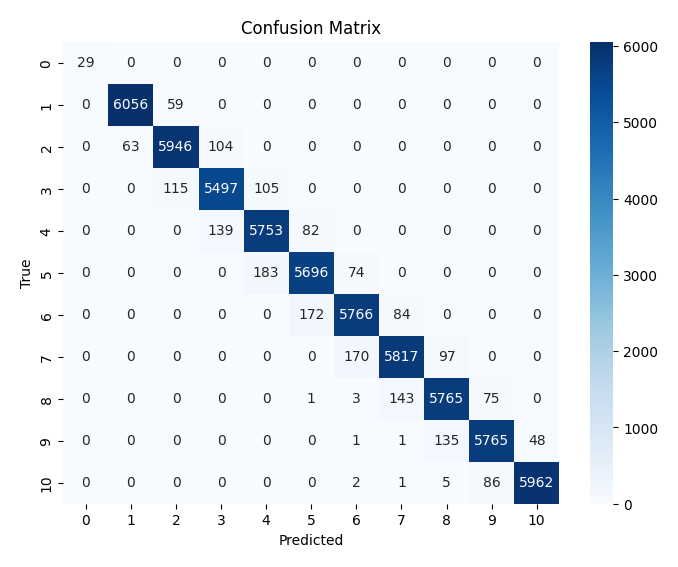
\includegraphics[width=0.72\linewidth]{pic/classification/random_forest.png}
    \vspace{0.5em}\caption{Матрица ошибок Случайного леса}
    \label{ris:forest-class}
\end{figure}
\vspace{1em}

\begin{figure}[H]
    \centering
    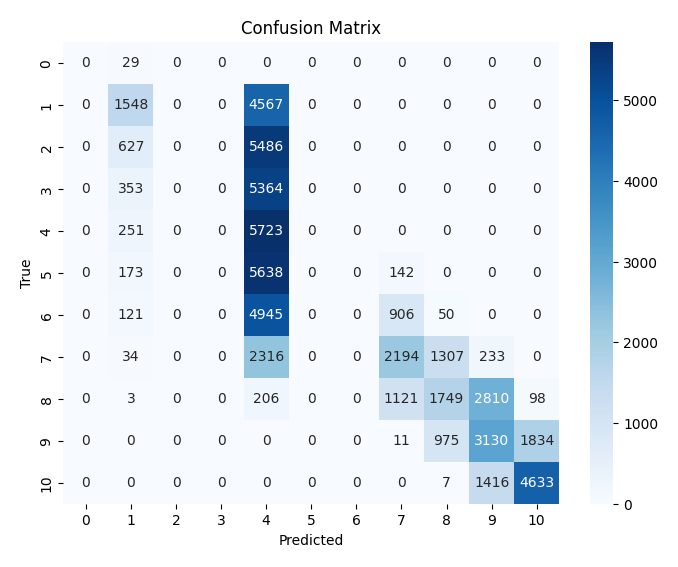
\includegraphics[width=0.72\linewidth]{pic/classification/adaboost.png}
    \vspace{0.5em}\caption{Матрица ошибок AdaBoost}
    \label{ris:adaboost-class}
\end{figure}

\newpage
\begin{flushright}
Окончание приложения Б
\end{flushright}
\vspace{-1.5em}

\begin{figure}[H]
    \centering
    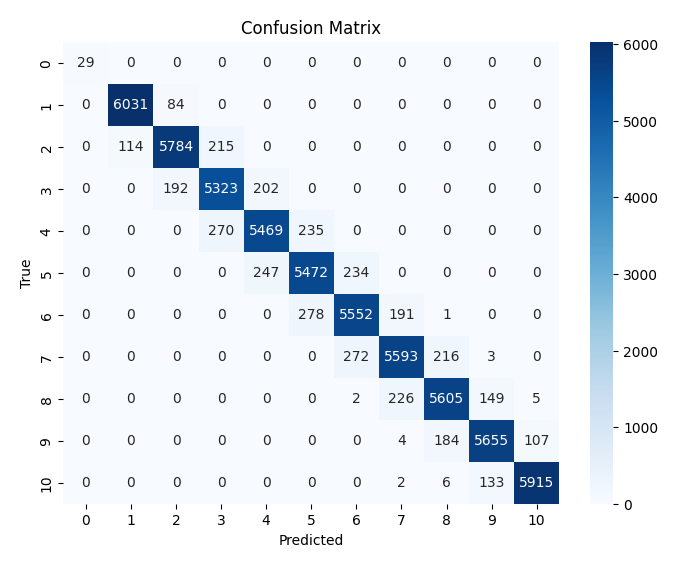
\includegraphics[width=0.75\linewidth]{pic/classification/decision_tree.png}
    \vspace{0.5em}\caption{Матрица ошибок Дерева решений}
    \label{ris:tree-class}
\end{figure}
\vspace{1em}

\begin{figure}[H]
    \centering
    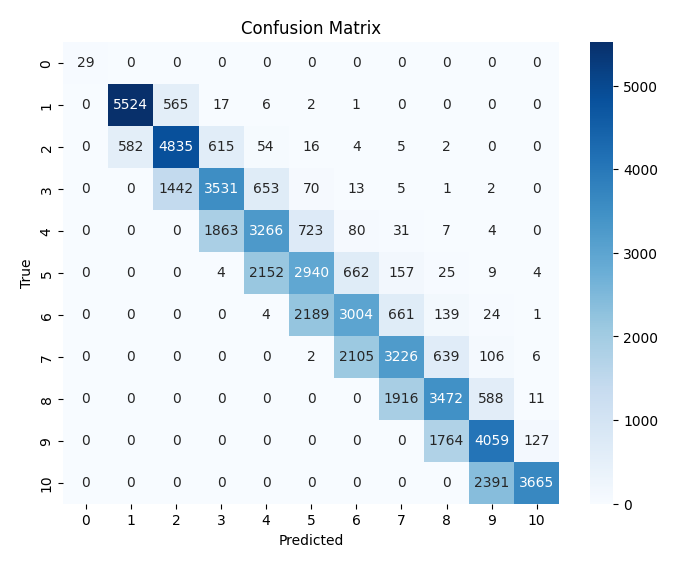
\includegraphics[width=0.75\linewidth]{pic/classification/naive_bayes.png}
    \vspace{0.5em}\caption{Матрица ошибок Наивного байесовского классификатора}
    \label{ris:bayes-class}
\end{figure}
\vspace{1em}

\newpage
\noindent \subsectionnonumber{Приложение В. Графики зависимостей}
\label{sec:graphics}

На рисунке~\ref{ris:tree-graph} представлен график зависимости времени выполнения и значений метрик от числа случайного распределения для Деревьев решений, а на рисунке~\ref{ris:boost-graph} представлена зависимость времени выполнения и значений метрик от числа базовых классификаторов Градиентного бустинга.

\begin{figure}[H]
    \centering
    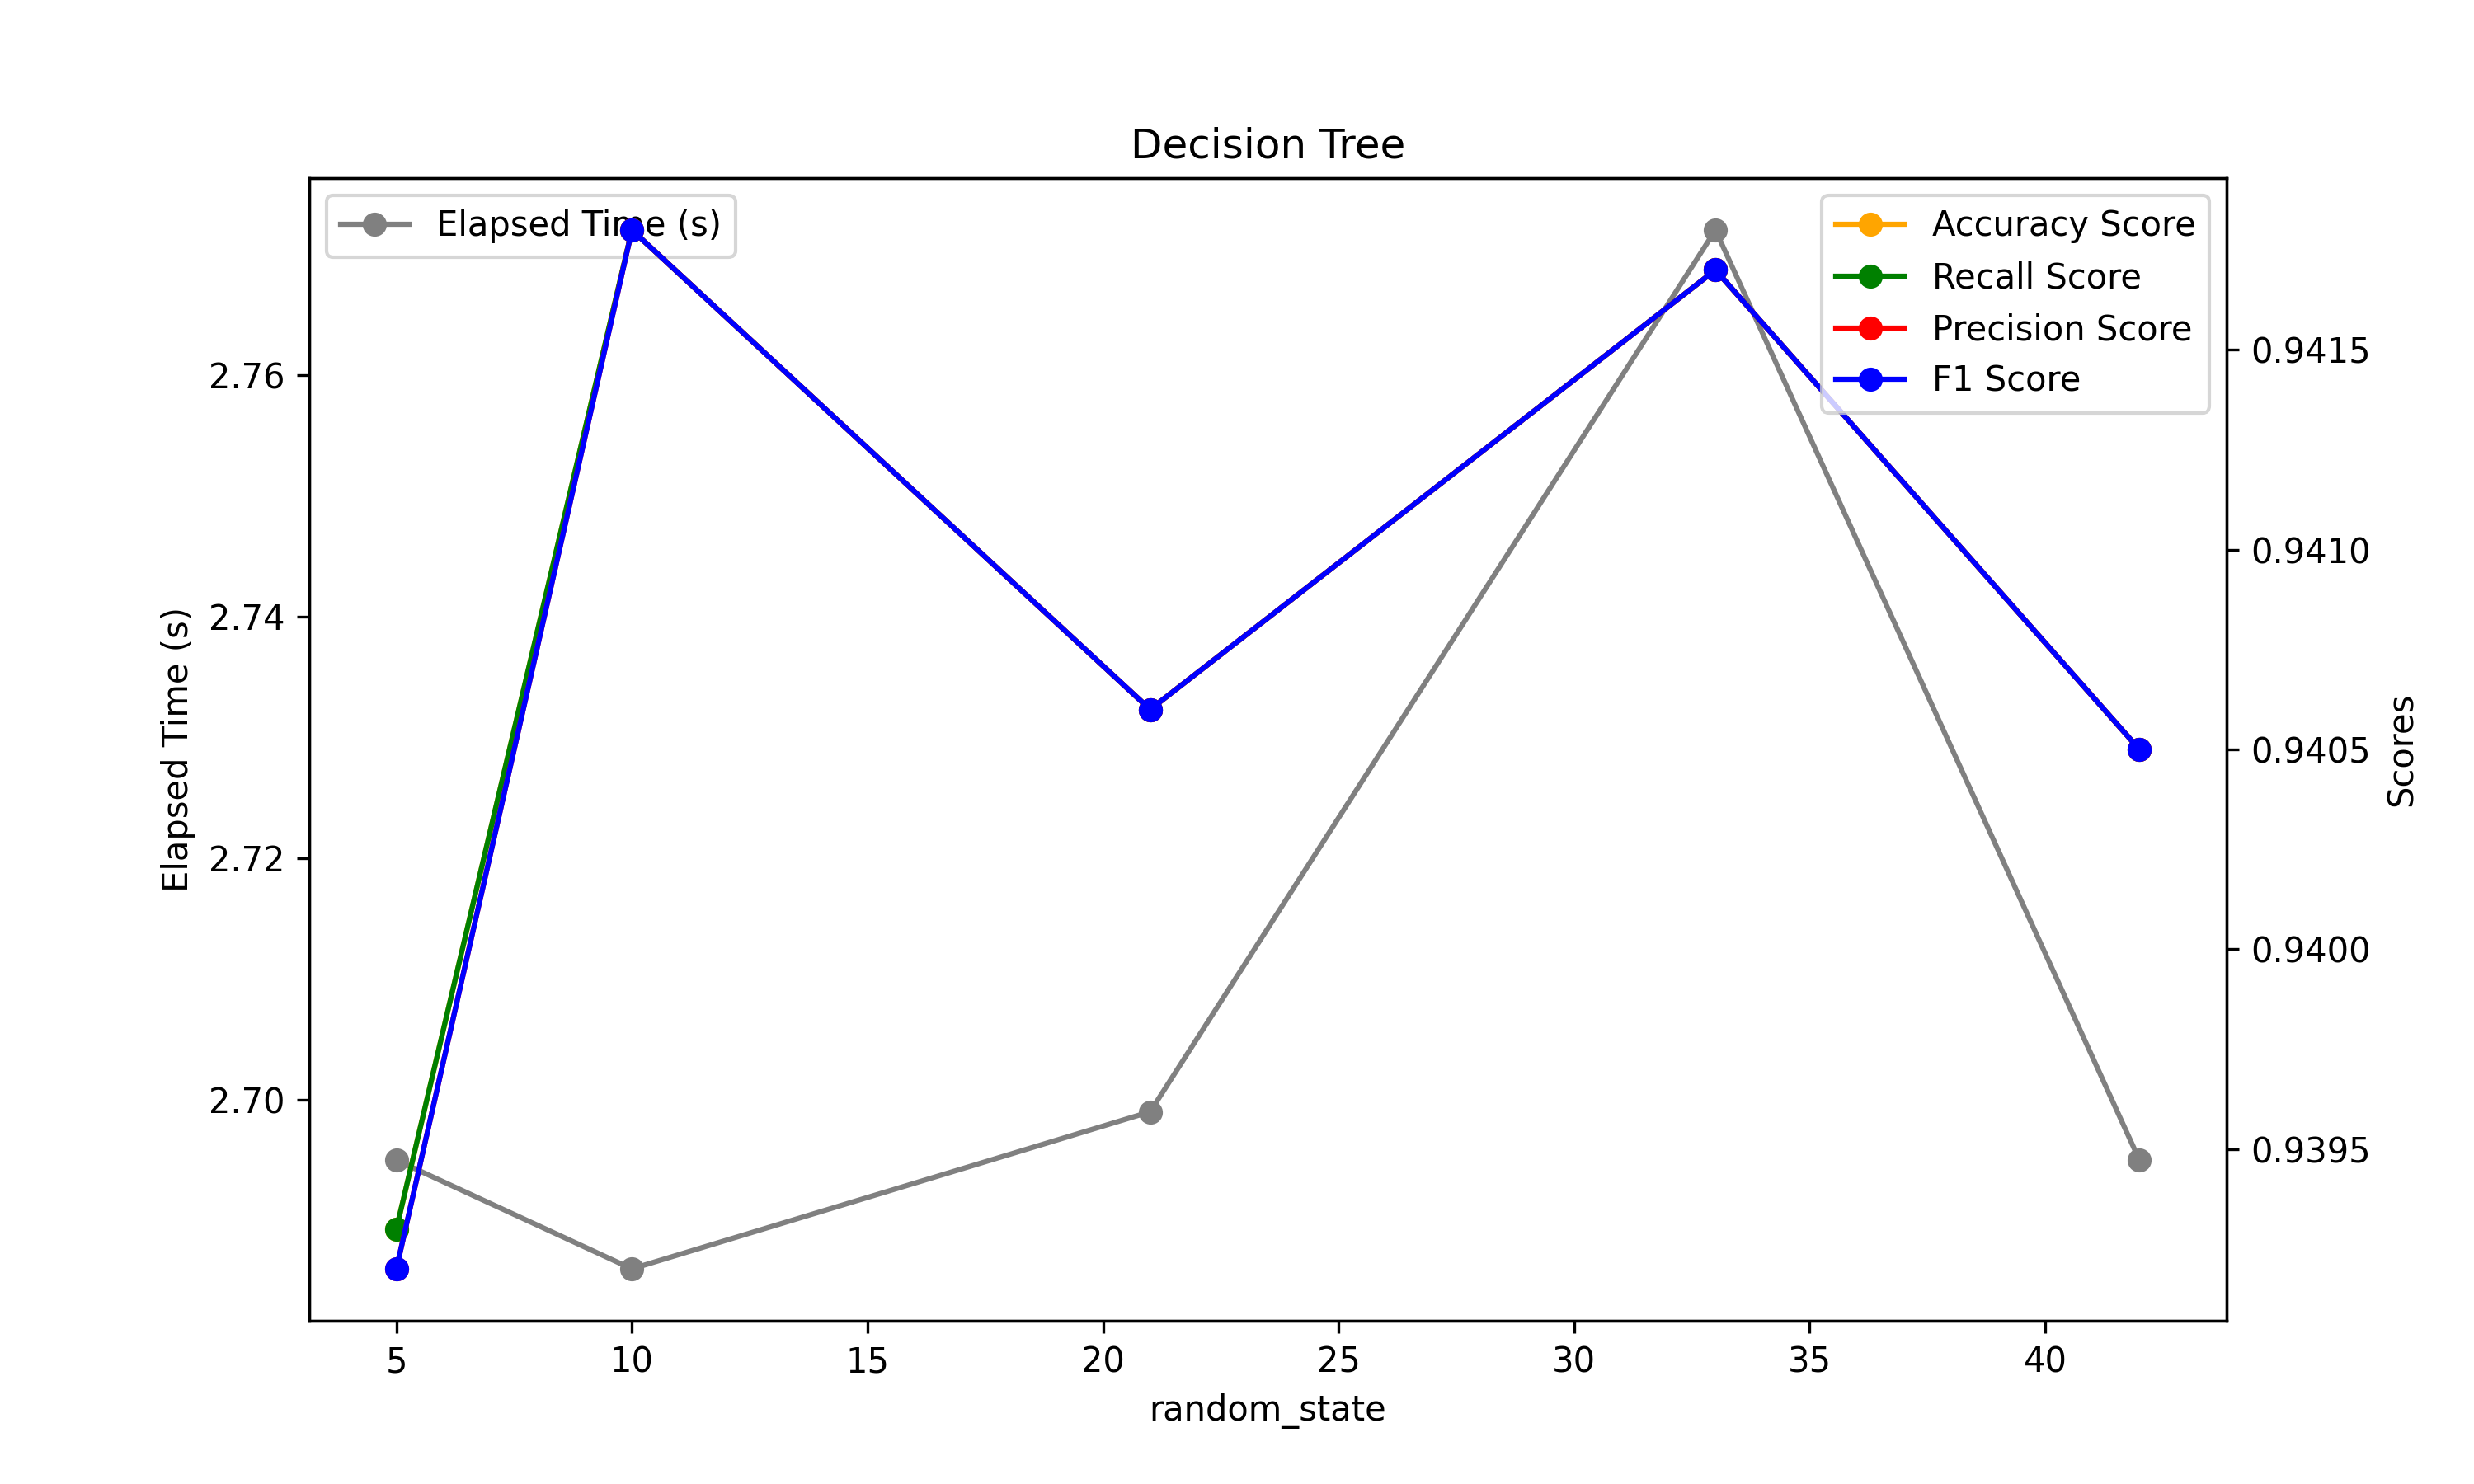
\includegraphics[width=0.9\linewidth]{pic/statistic/decision_tree.png}
    \vspace{0.2em}\caption{График зависимостей Дерева решений}
    \label{ris:tree-graph}
\end{figure}

\begin{figure}[H]
    \centering
    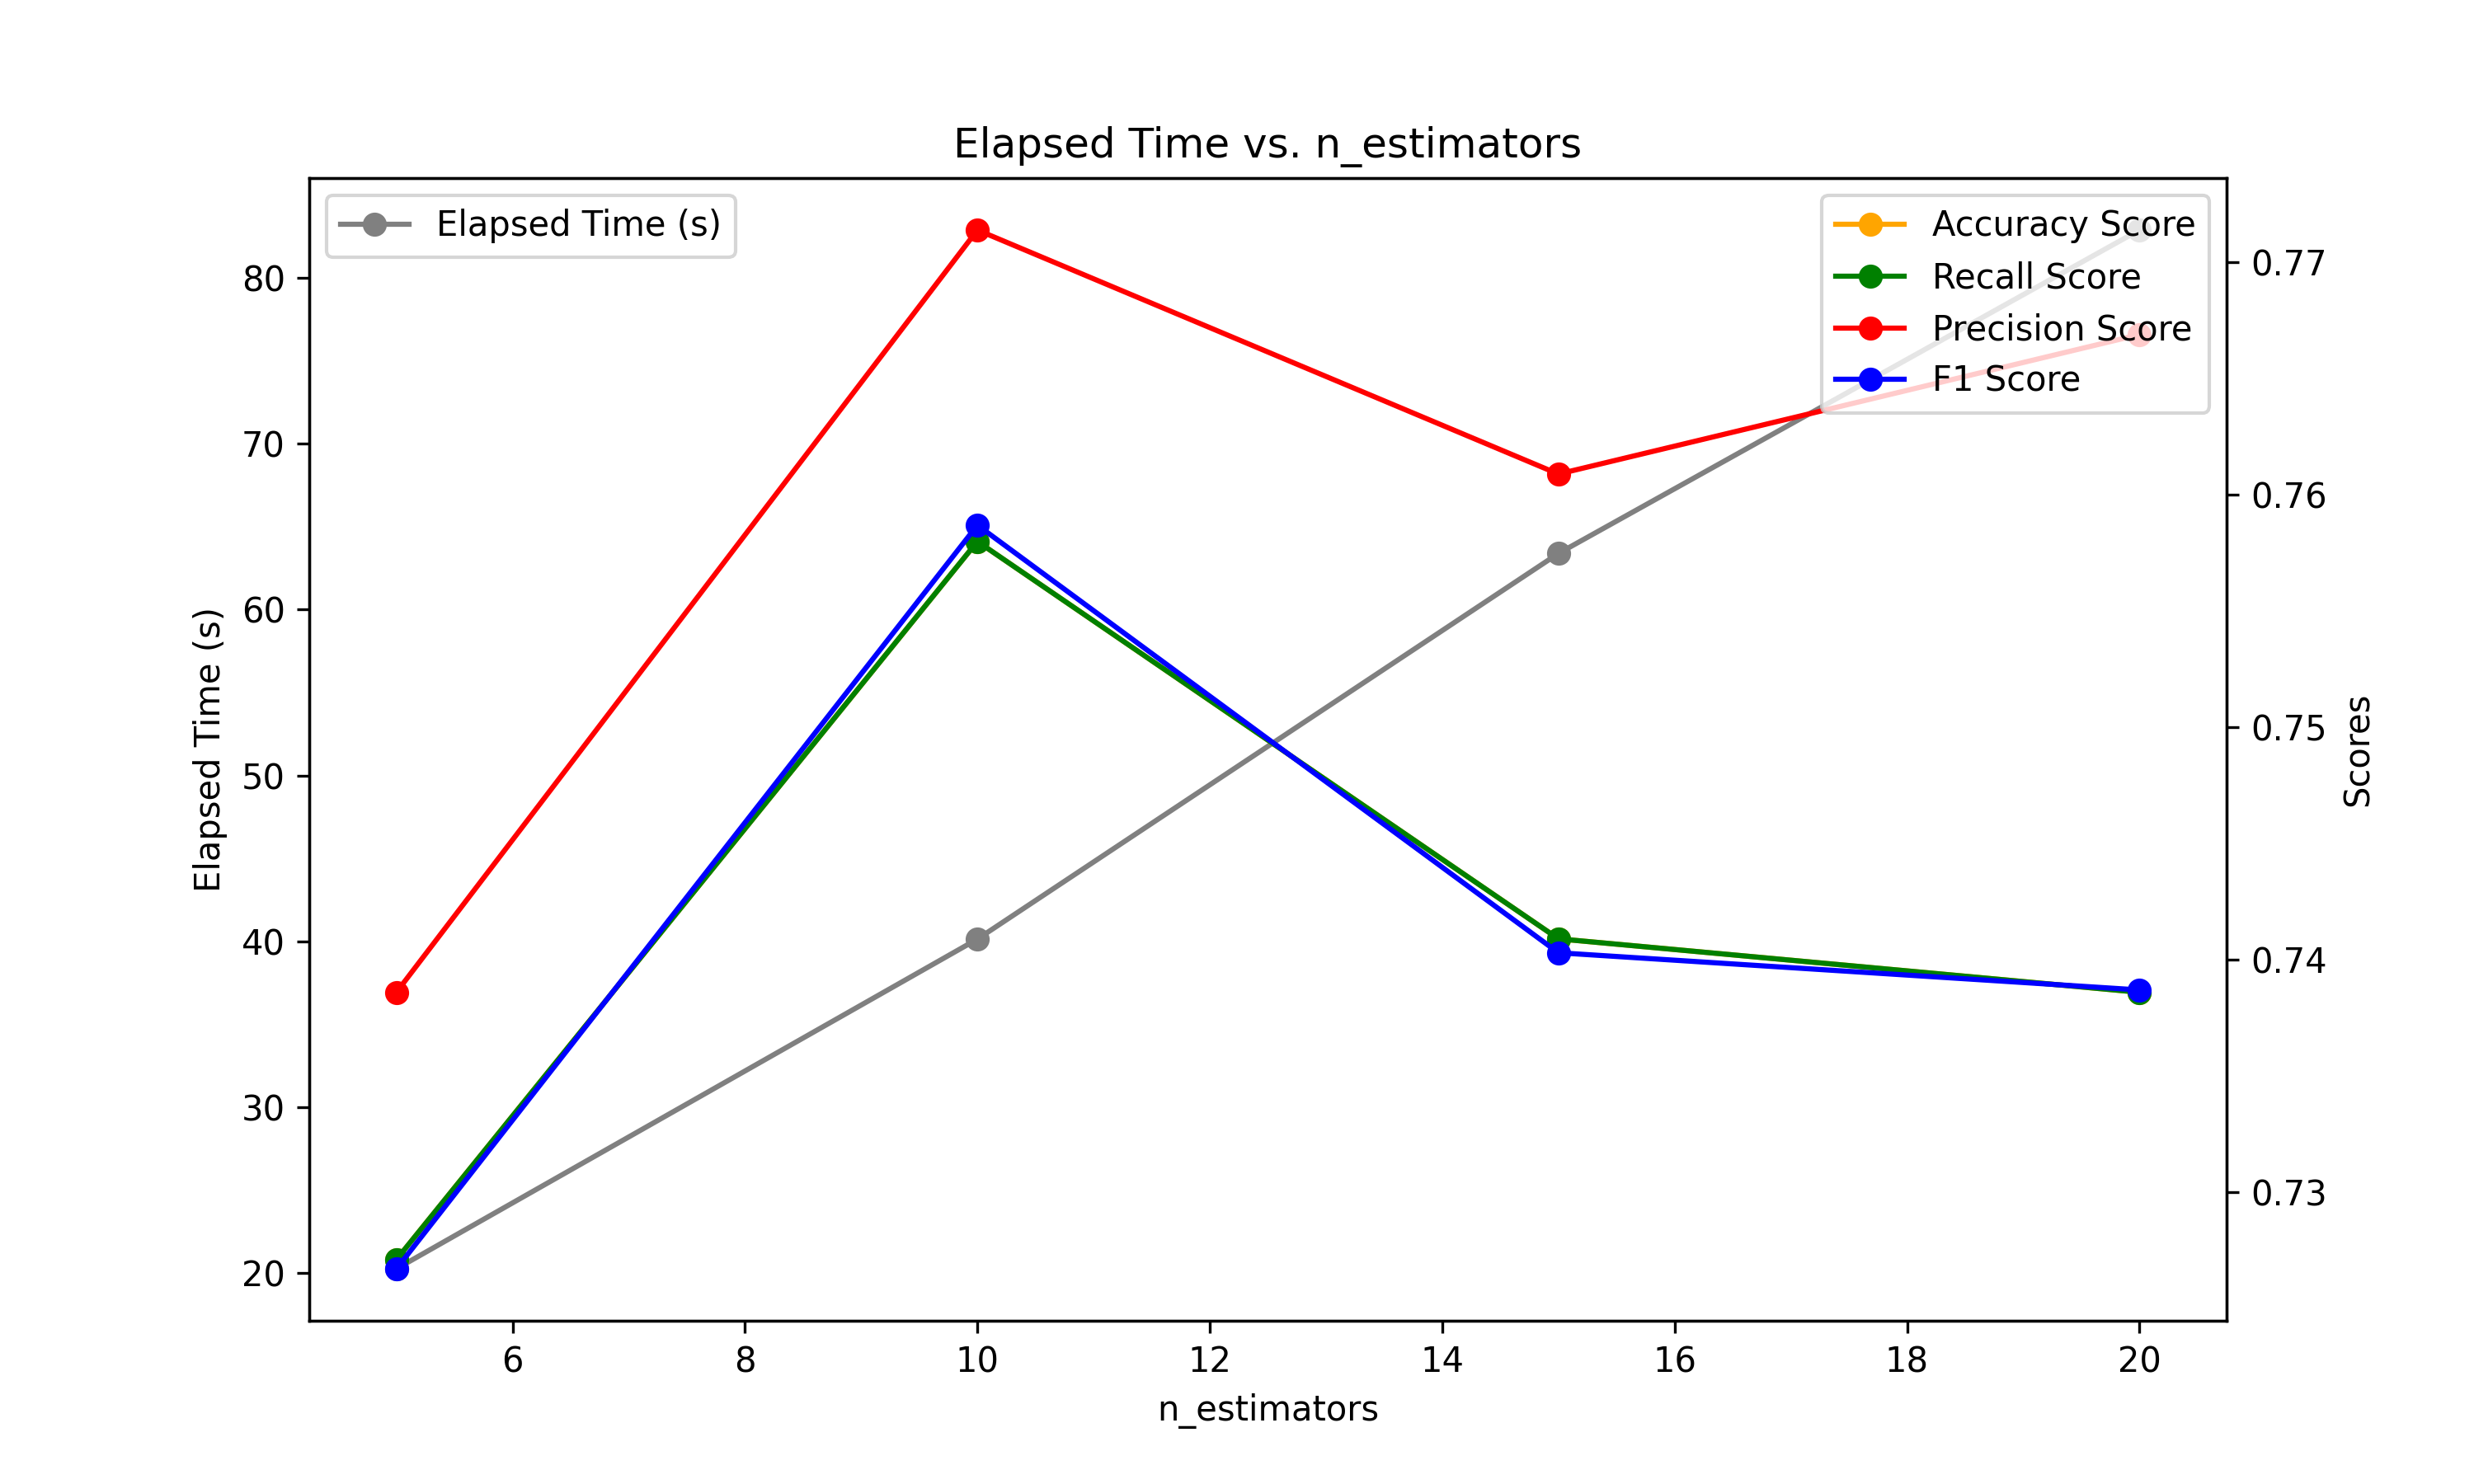
\includegraphics[width=0.9\linewidth]{pic/statistic/gradient_boosting.png}
    \vspace{0.2em}\caption{График зависимости Градиентного бустинга}
    \label{ris:boost-graph}
\end{figure}
\vspace{1em}

\newpage
\noindent \subsectionnonumber{Приложение Г. Тестирование определения}
\label{sec:test}
Для оценки качества работы классификации и регрессии были сформированы тестовые наборы, отражающие различные проекты GitHub с данными.

В таблице~\ref{tab:regr} представлен тестовый набор данных, где каждый объект характеризуется набором данных  (repo, forks, issues, commits, pull-requests, contributors) по проекту, на определенной модели. Ожидаемый результат определен вручную и показывает, какое существующее значение звезд имеется у проекта. Итоговый результат определяется в результате выполнения регрессии приложением.
\begin{table}[H]
    \setstretch{1.0}
    \caption{Определение звезд проекта по данным тестового набора}
    \fontsize{12pt}{1em}\selectfont
    \vspace{1em}
    \begin{tabularx}{\linewidth}{|c|l|X|X|X|}
       \hline
        № & Набор данных & Модель & Ожидае-мый результат & Итоговый результат \\ \hline
 1 & freeCodeCamp, 36178, 16557, 275, 61802, 185 & Gradient Boosting & 214813 &  141557 \\ \hline
 2 & freeCodeCamp, 36178, 16557, 275, 61802, 185 & Random Forest & 214813 &   168287 \\ \hline
 3 & the-art-of-command-line, 14268, 258, 54, 597, 42 & Gradient Boosting  & 128544 &  91454 \\ \hline
 4 & the-art-of-command-line, 14268, 258, 54, 597, 42 & Random Forest  & 128544 &  124194 \\ \hline
 5 & check, 250, 209, 3, 401, 2 & Gradient Boosting  & 1109 &   1073 \\ \hline
 6 & check, 250, 209, 3, 401, 2 & Random Forest  & 1109 &  1163 \\ \hline
 7 & postgres-operator, 1025, 1713, 645, 1453, 22 & Gradient Boosting  & 9324 & 6693 \\ \hline
 8 & postgres-operator, 1025, 1713, 645, 1453, 22 & Random Forest  & 9324 & 8714 \\ \hline
 9 & tweet-old-post, 25, 549, 8, 1083, 5 & Gradient Boosting  & 8 & 19 \\ \hline
 10 & tweet-old-post, 25, 549, 8, 1083, 5 & Random Forest  & 8 & 8 \\ \hline
 11 & sdk-dotnet, 191, 172, 6, 160, 1& Gradient Boosting  & 115 & 265 \\ \hline
 12 & sdk-dotnet, 191, 172, 6, 160, 1& Random Forest  & 115 & 341 \\ \hline
 13 & controller-topology-project, 20, 10, 2, 456, 2 & Gradient Boosting  & 8 & 25 \\ \hline
 14 & controller-topology-project, 20, 10, 2, 456, 2 & Random Forest  & 8 & 19 \\ \hline
        \end{tabularx} 
    \label{tab:regr}
\end{table}
\vspace{1em}

\newpage
\begin{flushright}
Окончание приложения Г
\end{flushright}
\vspace{0.5em}


В таблице~\ref{tab:class} представлен тестовый набор данных, где каждый объект характеризуется набором данных  (repo, forks, stars, issues, commits, pull-requests, contributors) по проекту, на определенной модели. Ожидаемый результат класса определен вручную и показывает, какое значение класса популярности имеется у проекта. Итоговый результат определяется в результате выполнения классификации приложением.
\begin{table}[H]
    \setstretch{1.0}
    \caption{Определение популярности по данным тестового набора}
    \fontsize{12pt}{1em}\selectfont
    \vspace{1em}
    \begin{tabularx}{\linewidth}{|c|l|X|X|X|}
       \hline
        № & Набор данных & Модель & Ожида-емый & Итого-вый \\ \hline
 1 & freeCodeCamp, 36178, 214813, 16557, 275, 61802, 185 & Gradient Boosting & 10 &  10 \\ \hline
 2 & freeCodeCamp, 36178, 214813, 16557, 275, 61802, 185 & Random Forest & 10 & 10 \\ \hline
 3 & freeCodeCamp, 36178, 214813, 16557, 275, 61802, 185 & Decision Tree & 10 & 10 \\ \hline
 4 & art-of-command-line, 14268, 128544, 258, 54, 597, 42 & Gradient Boosting  & 10 & 10  \\ \hline
 5 & art-of-command-line, 14268, 128544, 258, 54, 597, 42 & Random Forest & 10 & 10  \\ \hline
 6 & art-of-command-line, 14268, 128544, 258, 54, 597, 42 & Decision Tree  & 10 & 10  \\ \hline
 7 & check, 250, 1109, 209, 3, 401, 2 & Gradient Boosting  & 9 & 9 \\ \hline
 8 & check, 250, 1109, 209, 3, 401, 2 & Random Forest  & 9 & 9 \\ \hline
 9 & check, 250, 1109, 209, 3, 401, 2 & Decision Tree  & 9 & 9 \\ \hline
 10 & controller-topology-project, 20, 8, 10, 2, 456, 2 & Random Forest  & 8 & 8 \\ \hline
 11 & controller-topology-project, 20, 8, 10, 2, 456, 2 & Decision Tree  & 8 & 8 \\ \hline
 12 & myt-shard, 9, 5, 2, 1, 213, 1 & Gradient Boosting  & 6 & 6 \\ \hline
 13 & myt-shard, 9, 5, 2, 1, 213, 1 & Random Forest  & 6 & 6 \\ \hline
 14 & myt-shard, 9, 5, 2, 1, 213, 1 & Decision Tree  & 6 & 6 \\ \hline
 15 & DesignAndPrint, 1, 2, 18, 1, 6, 1 & Gradient Boosting  & 2 & 2 \\ \hline
 16 & DesignAndPrint, 1, 2, 18, 1, 6, 1 & Random Forest  & 2 & 2 \\ \hline
 17 & DesignAndPrint, 1, 2, 18, 1, 6, 1 & Decision Tree  & 2 & 2 \\ \hline
        \end{tabularx} 
    \label{tab:class}
\end{table}
\vspace{1em}
